%% Commands for TeXCount
%TC:macro \cite [option:text,text]
%TC:macro \citep [option:text,text]
%TC:macro \citet [option:text,text]
%TC:envir table 0 1
%TC:envir table* 0 1
%TC:envir tabular [ignore] word
%TC:envir displaymath 0 word
%TC:envir math 0 word
%TC:envir comment 0 0

%%
%% TKDD Submission: use "manuscript, screen, review, anonymous" for double-anonymous review
%% For final accepted version: \documentclass[acmsmall]{acmart}
%%
\documentclass[manuscript, screen, review, anonymous]{acmart}

%%
%% Journal metadata for TKDD
%%
\acmJournal{TKDD}
\acmVolume{0}
\acmNumber{0}
\acmArticle{0}
\acmYear{2026}
\acmDOI{XXXXXXX.XXXXXXX}

%%
%% Copyright — update when rights form is completed
%%
\setcopyright{acmlicensed}
\copyrightyear{2026}

%%
%% BibTeX command
%%
\AtBeginDocument{%
  \providecommand\BibTeX{{%
    Bib\TeX}}}

%%
%% Packages
%%
\usepackage{amsmath,amsfonts}
\usepackage{amsthm}
\usepackage{mathtools}
\usepackage{algorithm}
\usepackage[noend]{algorithmic}
\usepackage{array}
\usepackage{multirow}
\usepackage{subcaption}
\usepackage{tikz}
\usetikzlibrary{positioning, arrows.meta, calc, fit, backgrounds, shapes.geometric}

%%
%% Custom macros
%%
\newcommand{\cmark}{\textcolor{green!60!black}{\checkmark}}
\newcommand{\xmark}{\textcolor{red!70!black}{$\times$}}

\definecolor{bestcolor}{HTML}{D63384}
\definecolor{runnerup}{HTML}{B8860B}
\newcommand{\best}[1]{\textcolor{bestcolor}{\textbf{#1}}}
\newcommand{\runup}[1]{\textcolor{runnerup}{\underline{#1}}}

\newtheorem{proposition}{Proposition}
\newtheorem{remark}{Remark}


\begin{document}

%%
%% Title
%%
\title{PCGT: A Graph Transformer with Topology-Aware Partition Attention}

%%
%% Authors — ANONYMIZED for double-anonymous review
%% (Uncomment and fill in for camera-ready)
%%
% \author{Author 1}
% \affiliation{%
%   \institution{Institution}
%   \city{City}
%   \country{Country}
% }
% \email{author1@example.com}

%%
%% Abstract
%%
\begin{abstract}
Graph Transformers for node classification must choose between global attention at $O(N^2)$ cost and efficient kernel approximations that discard topology. We propose \textbf{PCGT} (Partition-Conditioned Graph Transformer), which sidesteps this tradeoff by operating at two attention resolutions. Exact softmax attention within graph partitions captures intra-community patterns, while learned seed vectors pool each partition into representatives for cross-partition global context. The model blends this partition-conditioned attention with a GCN backbone through learnable parameters---including an unconstrained self-connection weight $\beta$ that goes negative on heterophilic graphs, suppressing a node's own features when they conflict with its label.

On 14 benchmarks---including ogbn-arxiv (169K nodes) and pokec (1.6M nodes)---PCGT achieves statistically significant gains on heterophilic graphs ($+$3.8\% Chameleon, $+$3.8\% Squirrel over SGFormer), consistent improvements on homophilic datasets (CiteSeer $+$0.5\%, PubMed $+$0.6\%), and competitive scaling to million-node graphs. Ablations show that the attention mechanism's contribution grows with heterophily, and that each design choice---local attention, global seeds, partition encoding---adds measurable accuracy.
\end{abstract}

%%
%% CCS Classification
%%
\begin{CCSXML}
<ccs2012>
   <concept>
       <concept_id>10010147.10010257</concept_id>
       <concept_desc>Computing methodologies~Machine learning</concept_desc>
       <concept_significance>500</concept_significance>
   </concept>
   <concept>
       <concept_id>10010147.10010257.10010293.10010294</concept_id>
       <concept_desc>Computing methodologies~Neural networks</concept_desc>
       <concept_significance>500</concept_significance>
   </concept>
   <concept>
       <concept_id>10002951.10003317.10003347.10003356</concept_id>
       <concept_desc>Information systems~Clustering and classification</concept_desc>
       <concept_significance>300</concept_significance>
   </concept>
</ccs2012>
\end{CCSXML}

\ccsdesc[500]{Computing methodologies~Machine learning}
\ccsdesc[500]{Computing methodologies~Neural networks}
\ccsdesc[300]{Information systems~Clustering and classification}

%%
%% Keywords
%%
\keywords{graph transformers, node classification, graph partitioning, attention mechanisms, heterophilic graphs}

\maketitle

% ============================================================================
% 1. INTRODUCTION
% ============================================================================
\section{Introduction}
\label{sec:intro}

Why do the most accurate graph transformers remain the most expensive? Standard transformers compute all-pair attention over $N$ nodes at $O(N^2)$ cost, which captures global dependencies but is impractical beyond a few thousand nodes. Efficient alternatives---kernel approximations~\cite{wu2022nodeformer}, fixed linear projections~\cite{wu2023sgformer}, and random feature maps~\cite{wu2023difformer}---reduce cost to $O(N)$ but treat all node pairs uniformly, discarding the topology that makes graphs different from unstructured sets. This creates a fundamental tension: \emph{expressiveness} (topology-aware, exact attention) versus \emph{scalability} (subquadratic cost).

Graph neural networks (GNNs) based on message passing~\cite{gilmer2017mpnn, kipf2017semi, scarselli2009gnn} avoid the quadratic bottleneck by aggregating features from local neighborhoods. They achieve strong results on \emph{homophilic} graphs where connected nodes share similar labels, but struggle on \emph{heterophilic} graphs where neighbors frequently belong to different classes~\cite{zhu2020h2gcn, pei2020geomgcn}. Standard neighborhood aggregation blends features from dissimilar nodes, degrading representations~\cite{li2018oversmoothing}. Heterophily-specific GNNs (H$_2$GCN~\cite{zhu2020h2gcn}, GloGNN~\cite{li2022glognn}, GPR-GNN~\cite{chien2021gprgnn}) modify the aggregation scheme, but remain constrained to local or fixed-hop neighborhoods.

Real-world graphs exhibit \emph{multi-resolution} structure: nodes form local communities (captured by graph partitions) while also participating in global patterns (cross-community interactions). Local GNNs ignore the global patterns; single-resolution global transformers ignore the community structure. Exploiting both scales simultaneously, without incurring quadratic cost, remains an open challenge.

We propose \textbf{PCGT} (Partition-Conditioned Graph Transformer), which resolves this tension by operating at two attention resolutions simultaneously:
\begin{itemize}
\item \textbf{Fine (local):} Exact softmax attention within each graph partition, capturing detailed intra-community patterns at cost $O(N^2/K)$.
\item \textbf{Coarse (global):} Learned seed vectors attention-pool each partition into $M$ representative vectors; every node then cross-attends to all $KM$ representatives for global context at cost $O(NMK)$.
\item \textbf{Adaptive blending:} Learnable scalars $\alpha$ (local vs.\ global) and $\beta$ (unconstrained self-connection) allow the model to adapt to both homophilic and heterophilic regimes.
\end{itemize}

The key insight is that graph partitions (computed by METIS~\cite{karypis1998metis}) provide a \emph{natural} two-level hierarchy: nodes and communities. By restricting exact attention to within-partition scope and using learned pooling for cross-partition communication, PCGT achieves the expressiveness of exact attention where it matters most (within communities) while maintaining subquadratic global complexity.

Our contributions are:
\begin{enumerate}
\item A \textbf{multi-resolution partition attention} mechanism that is both topology-aware and subquadratic, combining the expressiveness of exact attention with the scalability of learned pooling (\S\ref{sec:method}).

\item An \textbf{unconstrained self-connection weight} $\beta$ that adapts per dataset---going negative on Film and Deezer where suppressing self-features helps, and strongly positive on feature-rich heterophilic graphs like Chameleon ($\beta = +3.08$) and Squirrel ($\beta = +3.53$). We provide an empirical analysis of this behavior and a gradient-based characterization of when $\beta^* < 0$ (\S\ref{sec:beta_analysis}).

\item \textbf{Experiments on 14 benchmarks}---including ogbn-arxiv (169K nodes), pokec (1.6M nodes), and Amazon2M (2.4M nodes)---where PCGT achieves statistically significant gains on heterophilic graphs ($+$3.8\% Chameleon, $+$3.8\% Squirrel over SGFormer), consistent improvements on homophilic datasets (CiteSeer $+$0.5\%, PubMed $+$0.6\%), and competitive performance on the remaining benchmarks (\S\ref{sec:results}).

\item An \textbf{analysis of partition strategies}: topology-aware (METIS) partitioning helps on structured heterophilic graphs, and ablations confirm that each component---local attention, global seeds, partition structural encoding (PSE), GCN branch---adds measurable accuracy (\S\ref{sec:ablation_results}).
\end{enumerate}


% ============================================================================
% 2. RELATED WORK
% ============================================================================
\section{Related Work}
\label{sec:related}

\textbf{Message-Passing GNNs.}~~The graph neural network framework~\cite{scarselli2009gnn, gilmer2017mpnn} aggregates features from local neighborhoods. GCN~\cite{kipf2017semi} and GAT~\cite{velickovic2018gat} aggregate features from immediate neighbors, performing well on homophilic graphs. APPNP~\cite{klicpera2019appnp} decouples feature transformation from propagation using personalized PageRank. SIGN~\cite{rossi2020sign} pre-computes multi-hop features for scalable inception-style aggregation. GIN~\cite{xu2019powerful} provides a maximally-expressive message passing framework. These methods are inherently local and struggle when informative nodes are distant or dissimilar to neighbors~\cite{li2018oversmoothing}.

\textbf{Heterophily-Specific GNNs.}~~H$_2$GCN~\cite{zhu2020h2gcn} addresses heterophily through ego/neighbor separation, higher-order neighborhoods, and intermediate representation combination. GloGNN~\cite{li2022glognn} learns a global coefficient matrix to capture correlations between all node pairs, with signed weights that can down-weight heterophilic neighbors. CPGNN~\cite{zhu2021cpgnn} uses compatibility matrices to model label-label correlations across edges. Geom-GCN~\cite{pei2020geomgcn} maps nodes to a latent geometric space to define aggregation neighborhoods. GPR-GNN~\cite{chien2021gprgnn} learns signed generalized PageRank weights to adaptively combine multi-hop information. While effective, these methods either require expensive global computation ($O(N^2)$ for GloGNN) or are limited to fixed neighborhood structures.

\textbf{Graph Transformers.}~~Transformers~\cite{vaswani2017attention} have been adapted for graphs to capture long-range dependencies beyond local neighborhoods. Graphormer~\cite{ying2021graphormer} incorporates structural and spatial encodings into standard transformer attention. GraphGPS~\cite{rampasek2022graphgps} provides a modular framework combining positional encodings~\cite{dwivedi2022lspe} with local and global attention. SAN~\cite{kreuzer2021rethinking} uses spectral attention with learned positional encodings. NodeFormer~\cite{wu2022nodeformer} uses Gumbel-softmax kernelized attention for $O(N)$ all-pair computation, but requires random feature approximation. DIFFormer~\cite{wu2023difformer} frames attention as energy-constrained diffusion. SGFormer~\cite{wu2023sgformer} achieves $O(N)$ global attention via a simplified single-layer, single-head design with a fixed kernel trick, demonstrating that deep multi-head attention is unnecessary for node classification on large graphs. Exphormer~\cite{shirzad2023exphormer} sparsifies attention using expander graphs and virtual nodes to achieve linear complexity; however, its attention pattern is fixed by the expander topology and the original paper does not report node classification results on the datasets we study, precluding direct experimental comparison without re-implementation. GOAT~\cite{kong2023goat} proposes global-local attention via $k$-hop neighborhood sampling, achieving scalability on large graphs; it operates in an inductive, sampling-based regime that differs from the full-graph transductive protocol we follow, making direct comparison non-trivial. Xing et al.~\cite{xing2024less} identify the ``over-globalizing'' problem in graph transformers and propose restricting attention scope---a concern that PCGT addresses via partition-conditioned locality. These methods are related in motivation to PCGT's partition-based approach, but none uses learned seed-based pooling to produce topology-aware inducing points.

\textbf{Partition-Based and Inducing Point Methods.}~~Graph partitioning via METIS~\cite{karypis1998metis} is widely used for distributed graph processing and mini-batch training~\cite{chiang2019clustergcn} but rarely integrated into the attention mechanism itself. Hierarchical graph pooling methods like DiffPool~\cite{ying2018hierarchical} and MinCutPool~\cite{bianchi2020mincut} learn coarsened graph representations but target graph-level tasks rather than node classification. Set Transformer~\cite{lee2019set} introduces learnable inducing points for efficient set-level attention in $O(NM)$, but these points are not topology-aware. PCGT combines these two lines of work: graph partitions define \emph{topology-aware} attention scopes, and learned seeds produce partition representatives through attention pooling.

\textbf{Positioning of PCGT.}~~Table~\ref{tab:positioning} contrasts PCGT with representative methods. Unlike SGFormer's single-resolution global kernel, PCGT operates at \emph{two} resolutions---exact local attention within partitions and learned cross-partition attention---exploiting the multi-scale structure of real graphs. Unlike GloGNN's $O(N^2)$ global coefficient matrix, PCGT achieves subquadratic complexity via partition-conditioned computation. Unlike Set Transformer's generic inducing points, PCGT's representatives are grounded in graph topology through METIS partitioning and partition structural encoding.

\begin{table}[t]
\caption{Comparison of representative methods across key properties. PCGT uniquely combines multi-resolution attention with topology-aware partitioning.}
\label{tab:positioning}
\centering
\small
\begin{tabular}{l|cccc}
\toprule
\textbf{Property} & \textbf{GCN} & \textbf{GloGNN} & \textbf{SGFormer} & \textbf{PCGT} \\
\midrule
Scope & Local & Global & Global & Multi-res. \\
Complexity & $O(|E|)$ & $O(N^2)$ & $O(N)$ & $O(\frac{N^2}{K}\!+\!NMK)$ \\
Topology-aware & \cmark & \xmark & \xmark & \cmark \\
Heterophily & \xmark & \cmark & Partial & \cmark \\
Exact attention & \xmark & N/A & \xmark & \cmark\,(local) \\
\bottomrule
\end{tabular}
\end{table}


% ============================================================================
% 3. METHOD
% ============================================================================
\section{Method}
\label{sec:method}

\subsection{Overview and Architecture}

PCGT combines local and global attention with learnable blending (Figure~\ref{fig:architecture}). Given a graph with $N$ nodes, we: (1)~partition into $K$ approximately balanced regions (METIS), (2)~compute local attention within partitions at $O(N^2/K)$ cost, (3)~compute global attention via learned seeds at $O(N{\cdot}M{\cdot}K)$ cost, (4)~blend via learnable $\alpha$, (5)~weight self-connections via learnable $\beta$, and (6)~fuse with a GCN backbone for edge-level structural features.

\begin{figure*}[t]
\centering
\resizebox{\textwidth}{!}{%
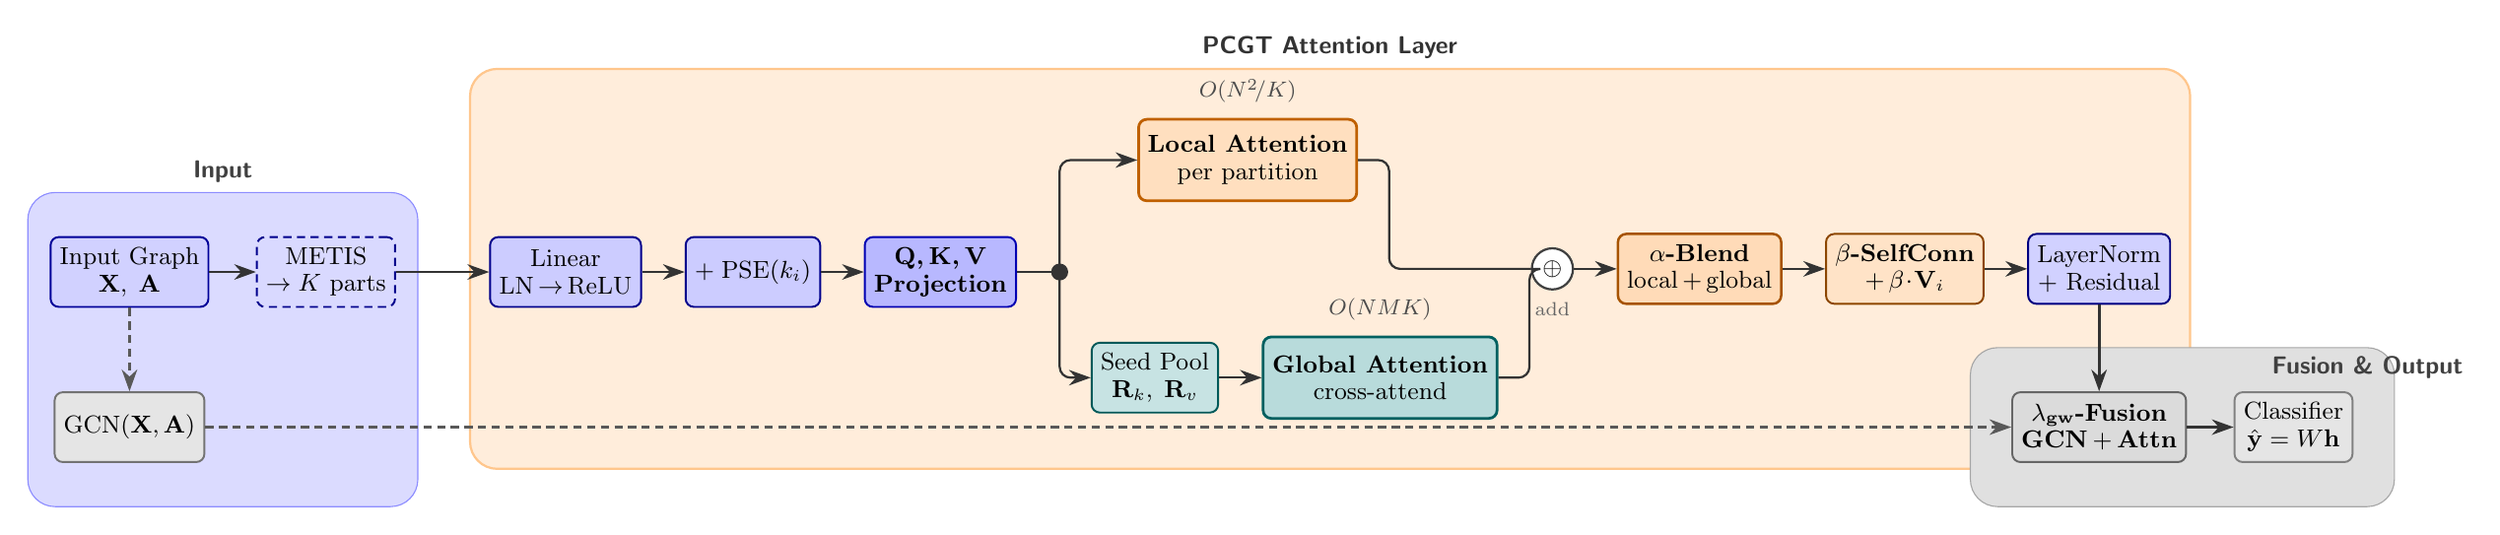
\begin{tikzpicture}[
  >={Stealth[length=2.8mm, width=2mm]},
  box/.style={
    draw, rounded corners=3pt, minimum height=0.90cm, minimum width=1.4cm,
    align=center, font=\small, line width=0.7pt,
  },
  inputbox/.style={box, fill=blue!18, draw=blue!60!black, minimum width=1.7cm},
  partbox/.style={box, fill=blue!15, draw=blue!55!black, minimum width=1.5cm, densely dashed},
  projbox/.style={box, fill=blue!20, draw=blue!55!black},
  qkvbox/.style={box, fill=blue!28, draw=blue!70!black, font=\small\bfseries},
  normbox/.style={box, fill=blue!18, draw=blue!50!black},
  localbox/.style={box, fill=orange!25, draw=orange!75!black, line width=1.0pt,
                   minimum width=2.2cm, minimum height=1.05cm},
  seedbox/.style={box, fill=teal!22, draw=teal!70!black, minimum width=1.6cm},
  globalbox/.style={box, fill=teal!28, draw=teal!75!black, line width=1.0pt,
                    minimum width=2.2cm, minimum height=1.05cm},
  blendbox/.style={box, fill=orange!28, draw=orange!65!black, line width=0.9pt},
  selfbox/.style={box, fill=orange!22, draw=orange!55!black},
  gcnbox/.style={box, fill=black!10, draw=black!55, minimum width=1.6cm},
  gwbox/.style={box, fill=black!14, draw=black!60, minimum width=1.6cm,
                font=\small\bfseries},
  outbox/.style={box, fill=black!10, draw=black!50, minimum width=1.5cm},
  arr/.style={->, line width=0.8pt, color=black!80},
  arrfork/.style={line width=0.8pt, color=black!80},
  gcnarr/.style={->, line width=1.0pt, color=black!65, densely dashed},
  stagelabel/.style={font=\small\bfseries\sffamily, text=black!80},
  complabel/.style={font=\footnotesize, text=black!70},
  forkdot/.style={circle, fill=black!80, inner sep=2.2pt},
  mergenode/.style={circle, draw=black!75, line width=0.8pt, inner sep=2pt,
                    font=\small, fill=white},
]

% === ROW 1: main transformer pipeline ===
\node[inputbox] (input) {Input Graph\\[-1pt]$\mathbf{X},\;\mathbf{A}$};
\node[partbox, right=0.6cm of input] (metis) {METIS\\[-1pt]$\to K$ parts};
\draw[arr] (input) -- (metis);
\node[projbox, right=1.2cm of metis] (linproj) {Linear\\[-1pt]LN\,$\to$\,ReLU};
\draw[arr] (metis) -- (linproj);
\node[projbox, right=0.55cm of linproj, minimum width=1.6cm] (pse) {$+\;\text{PSE}(k_i)$};
\draw[arr] (linproj) -- (pse);
\node[qkvbox, right=0.55cm of pse] (qkv) {Q,\,K,\,V\\[-1pt]Projection};
\draw[arr] (pse) -- (qkv);

\coordinate[right=0.55cm of qkv] (fork);
\node[forkdot] at (fork) {};
\draw[arrfork] (qkv) -- (fork);

\node[localbox, above right=0.9cm and 1.0cm of fork] (local) {%
  \textbf{Local Attention}\\[-1pt]
  {\small per partition}};
\node[complabel, above=2pt of local.north] {$O(N^2\!/K)$};
\draw[arr, rounded corners=4pt] (fork) |- (local);

\node[seedbox, below right=0.9cm and 0.4cm of fork] (seedpool) {Seed Pool\\[-1pt]$\mathbf{R}_k,\;\mathbf{R}_v$};
\draw[arr, rounded corners=4pt] (fork) |- (seedpool);
\node[globalbox, right=0.55cm of seedpool] (global) {%
  \textbf{Global Attention}\\[-1pt]
  {\small cross-attend}};
\node[complabel, above=2pt of global.north] {$O(NMK)$};
\draw[arr] (seedpool) -- (global);

\coordinate (mergeY) at ($(local.east)!0.5!(global.east)$);
\node[mergenode] (mergeN) at ($(mergeY) + (1.6,0)$) {$\oplus$};
\node[font=\scriptsize, text=black!60, below=1pt of mergeN] {add};
\draw[line width=0.8pt, color=black!80, rounded corners=4pt]
  (local.east) -- ++(0.4,0) |- (mergeN);
\draw[line width=0.8pt, color=black!80, rounded corners=4pt]
  (global.east) -- ++(0.4,0) |- (mergeN);

\node[blendbox, right=0.55cm of mergeN] (blend)
  {$\alpha$\textbf{-Blend}\\[-1pt]{\small local\,+\,global}};
\draw[arr] (mergeN) -- (blend);
\node[selfbox, right=0.55cm of blend] (self) {$\beta$\textbf{-SelfConn}\\[-1pt]$+\,\beta\!\cdot\!\mathbf{V}_i$};
\draw[arr] (blend) -- (self);
\node[normbox, right=0.55cm of self] (ln) {LayerNorm\\[-1pt]$+$ Residual};
\draw[arr] (self) -- (ln);

% === ROW 2: GCN branch + Fusion + Classifier ===
\node[gcnbox] (gcn) at ($(input) + (0,-2.0)$) {$\text{GCN}(\mathbf{X},\mathbf{A})$};
\draw[gcnarr] (input) -- (gcn);
\node[gwbox] (gwfuse) at (ln |- gcn) {$\lambda_{\text{gw}}$\textbf{-Fusion}\\[-1pt]{\small GCN\,$+$\,Attn}};
\draw[arr, line width=1.0pt] (ln) -- (gwfuse);
\draw[gcnarr] (gcn) -- (gwfuse);
\node[outbox, right=0.6cm of gwfuse] (output) {Classifier\\[-1pt]$\hat{\mathbf{y}} = W\mathbf{h}$};
\draw[arr] (gwfuse) -- (output);

% === Background regions ===
\begin{scope}[on background layer]
  \node[
    fill=blue!14, draw=blue!45, rounded corners=10pt,
    inner xsep=8pt, inner ysep=16pt,
    fit=(input)(metis)(gcn),
    label={[stagelabel, text=black!75]above:\textsf{Input}}
  ] {};
  \node[
    fill=orange!14, draw=orange!45, rounded corners=10pt,
    inner xsep=7pt, inner ysep=18pt, line width=0.8pt,
    fit=(linproj)(pse)(qkv)(local)(global)(seedpool)(blend)(self)(ln),
    label={[stagelabel, text=black!80]above:\textsf{PCGT Attention Layer}}
  ] {};
  \node[
    fill=black!12, draw=black!35, rounded corners=10pt,
    inner xsep=15pt, inner ysep=16pt,
    fit=(gwfuse)(output),
    label={[stagelabel, text=black!75, anchor=north west]above right:\textsf{Fusion \& Output}}
  ] {};
\end{scope}

\end{tikzpicture}
}% end resizebox
\caption{Architecture of PCGT\@. The input graph is partitioned via METIS into $K$ groups. Node features are linearly projected, augmented with partition structural encoding (PSE), then Q/K/V projections feed two parallel branches: \emph{local attention} within each partition (using Q, K, V restricted to the partition) and \emph{global attention} where learned seeds pool each partition's K, V into representatives $\mathbf{R}_k, \mathbf{R}_v$, and every node's Q cross-attends to all representatives. The branches are $\alpha$-blended, augmented with a $\beta$-weighted self-connection, and fused with a GCN branch via the graph-weight $\lambda_{\text{gw}}$.}
\label{fig:architecture}
\end{figure*}

\subsection{Local Attention and Partition Encoding}

Partition the graph into $K$ disjoint sets $\{S_1, \ldots, S_K\}$ using METIS. For partition $p$, compute exact softmax attention:
\begin{equation}
\text{Attn}_{\text{local}}^{(p)} = \text{softmax}\!\left( \frac{\mathbf{Q}[S_p] \mathbf{K}[S_p]^T}{\sqrt{d}} \right) \mathbf{V}[S_p],\; O(N^2\!/K)
\end{equation}

Partition structural encoding (PSE) is added before Q/K/V projection: $\mathbf{x}_i \leftarrow \mathbf{x}_i + \mathbf{E}_{k_i}$, where $\mathbf{E} \in \mathbb{R}^{K \times d}$ is a learned embedding table indexed by partition id $k_i$, initialized from $\mathcal{N}(0, 0.02)$. Unlike positional encodings~\cite{dwivedi2022lspe} that encode a node's position in the graph spectrum, PSE encodes \emph{which community} a node belongs to---a coarser structural signal that informs the attention mechanism about partition membership. PSE is added once (before projection) so that queries, keys, and values all carry this signal.

\subsection{Global Attention via Learned Seeds}
\label{sec:global_attn}

We learn $M$ seed query vectors $\mathbf{S} \in \mathbb{R}^{M \times d}$ shared across all partitions. For each partition $p$, the seeds attention-pool the partition's keys and values into $M$ representatives:
\begin{equation}
\mathbf{R}_k^{(p)} = \mathrm{softmax}\!\left( \frac{\mathbf{S} \, \mathbf{K}[S_p]^T}{\sqrt{d}} \right) \mathbf{K}[S_p], \quad \mathbf{R}_v^{(p)} = \mathrm{softmax}\!\left( \frac{\mathbf{S} \, \mathbf{K}[S_p]^T}{\sqrt{d}} \right) \mathbf{V}[S_p]
\label{eq:reps}
\end{equation}
where $\mathbf{R}_k^{(p)}, \mathbf{R}_v^{(p)} \in \mathbb{R}^{M \times d}$. Stacking across all $K$ partitions yields $\mathbf{R}_k, \mathbf{R}_v \in \mathbb{R}^{KM \times d}$. Each node then cross-attends to all representatives:
\begin{equation}
\text{Attn}_{\text{global}} = \text{softmax}\left( \frac{\mathbf{Q} \, \mathbf{R}_k^T}{\sqrt{d}} \right) \mathbf{R}_v, \quad O(N \cdot M \cdot K)
\end{equation}

This two-step design (pool then cross-attend) is related to inducing points in Set Transformer~\cite{lee2019set}, but our seeds are \emph{topology-aware}: they pool from graph-partitioned node groups rather than arbitrary subsets, and adapt to the task unlike the fixed kernel in SGFormer~\cite{wu2023sgformer}.

\subsection{Blending, Self-Connection, and GCN Fusion}

The local and global outputs are blended with a learnable scalar $\alpha = \sigma(\alpha_{\text{logit}})$ where $\sigma$ is the sigmoid function:
\begin{equation}
\mathbf{h}_{\text{context}} = \alpha \cdot \text{Attn}_{\text{local}} + (1 - \alpha) \cdot \text{Attn}_{\text{global}}
\end{equation}

A learnable self-connection weight $\beta \in \mathbb{R}$ (unconstrained) adds the node's own transformed value:
\begin{equation}
\mathbf{h}_{\text{attn}} = \mathbf{h}_{\text{context}} + \beta \cdot \mathbf{V}_i
\end{equation}

Because $\beta$ is \emph{unconstrained}, it can become negative. On datasets where a node's own features are less informative than the attention context (e.g., Film, Deezer), this lets the model suppress the self-connection. Conversely, on feature-rich graphs like Chameleon and Squirrel, $\beta$ grows strongly positive. We formalize this behavior in \S\ref{sec:beta_analysis}.

Finally, the PCGT attention output is fused with a GCN branch via a fixed hyperparameter $\lambda_{\text{gw}} \in [0,1]$:
\begin{equation}
\mathbf{h}_{\text{final}} = \lambda_{\text{gw}} \cdot \text{GCN}(\mathbf{X}, \mathbf{A}) + (1 - \lambda_{\text{gw}}) \cdot \mathbf{h}_{\text{attn}}
\end{equation}
where GCN is a standard multi-layer graph convolutional network~\cite{kipf2017semi}. The GCN branch provides explicit edge-level structural features that complement the partition-based attention.

The complete PCGT layer applies: input projection $\to$ PSE $\to$ Q,K,V projections $\to$ local + global attention $\to$ $\alpha$-blend $\to$ $\beta$ self-connection $\to$ LayerNorm $\to$ residual connection $\to$ dropout.

\begin{algorithm}[t]
\caption{PCGT Forward Pass (one layer)}
\label{alg:pcgt}
\begin{algorithmic}[1]
\REQUIRE Features $\mathbf{X} \in \mathbb{R}^{N \times d}$, adjacency $\mathbf{A}$, partitions $\{S_1, \ldots, S_K\}$
\ENSURE Updated features $\mathbf{H} \in \mathbb{R}^{N \times d}$
\STATE $\mathbf{X} \leftarrow \mathbf{X} + \mathbf{E}[\text{partition id}]$ \hfill \textit{// PSE lookup}
\STATE $\mathbf{Q}, \mathbf{K}, \mathbf{V} \leftarrow \mathbf{X} W_Q,\; \mathbf{X} W_K,\; \mathbf{X} W_V$
\FOR{$p = 1$ \textbf{to} $K$}
  \STATE $\mathbf{h}^{(p)}_{\mathrm{local}} \leftarrow \mathrm{softmax}\!\bigl(\mathbf{Q}[S_p]\, \mathbf{K}[S_p]^{\!\top}\!/\sqrt{d}\bigr)\, \mathbf{V}[S_p]$
  \STATE $\mathbf{R}_k^{(p)},\, \mathbf{R}_v^{(p)} \leftarrow \mathrm{SeedPool}(\mathbf{S},\, \mathbf{K}[S_p],\, \mathbf{V}[S_p])$
\ENDFOR
\STATE Stack $\mathbf{h}_{\mathrm{local}} \!\in\! \mathbb{R}^{N \times d}$;\; stack $\mathbf{R}_k, \mathbf{R}_v \!\in\! \mathbb{R}^{KM \times d}$
\STATE $\mathbf{h}_{\mathrm{global}} \leftarrow \mathrm{softmax}\!\bigl(\mathbf{Q}\, \mathbf{R}_k^{\!\top}\!/\sqrt{d}\bigr)\, \mathbf{R}_v$
\STATE $\mathbf{h}_{\mathrm{ctx}} \leftarrow \sigma(\alpha)\, \mathbf{h}_{\mathrm{local}} + (1\!-\!\sigma(\alpha))\, \mathbf{h}_{\mathrm{global}}$
\STATE $\mathbf{h}_{\mathrm{attn}} \leftarrow \mathbf{h}_{\mathrm{ctx}} + \beta \cdot \mathbf{V}$
\STATE $\mathbf{H} \leftarrow \lambda_{\mathrm{gw}}\, \mathrm{GCN}(\mathbf{X}, \mathbf{A}) + (1\!-\!\lambda_{\mathrm{gw}})\, \mathrm{LN}(\mathbf{h}_{\mathrm{attn}})$
\RETURN $\mathbf{H}$
\end{algorithmic}
\end{algorithm}

\subsection{Complexity Analysis}
\label{sec:complexity}

We derive the per-layer computational complexity of PCGT. Let $N$ be the number of nodes, $K$ the number of partitions, $M$ the number of seeds per partition, $d$ the hidden dimension, and $|E|$ the number of edges.

\textbf{Local attention.}~~For a balanced partition, each group contains approximately $N/K$ nodes. Standard self-attention within one partition costs $O((N/K)^2 \cdot d)$. Summing over all $K$ partitions:
\begin{equation}
C_\text{local} = K \cdot O\!\left(\frac{N^2 d}{K^2}\right) = O\!\left(\frac{N^2 d}{K}\right)
\end{equation}

\textbf{Seed pooling.}~~For each of the $K$ partitions, the $M$ seed queries attend over $N/K$ keys, costing $O(MNd/K)$ per partition and $O(MNd)$ total.

\textbf{Global cross-attention.}~~Each of the $N$ node queries attends over $KM$ representative keys:
\begin{equation}
C_\text{global} = O(N \cdot KM \cdot d)
\end{equation}

\textbf{GCN branch.}~~The multi-layer GCN costs $O(|E| \cdot d)$ per layer.

\textbf{Total per layer:}
\begin{equation}
C_\text{PCGT} = \underbrace{O\!\left(\frac{N^2 d}{K}\right)}_{\text{local attn}} + \underbrace{O(NMKd)}_{\text{global attn + pool}} + \underbrace{O(|E|d)}_{\text{GCN}}
\end{equation}

For typical settings ($N$=10K, $K$=10, $M$=4): $N^2/K = 10$M and $NMK = 400$K, giving ${\sim}10.4$M operations vs.\ ${\sim}100$M for full $O(N^2)$ attention---a ${\sim}10\times$ reduction. For ogbn-arxiv ($N$=169K, $K$=256, $M$=4): the total is ${\sim}285$M vs.\ 28.6B for full attention---a ${\sim}100\times$ reduction. We note that this comparison is against a theoretical $O(N^2)$ baseline; in practice, efficient graph transformers such as SGFormer already achieve $O(N)$ complexity. PCGT's overhead relative to SGFormer is 1.7--5.0$\times$ on most datasets (Table~\ref{tab:runtime}), which is the practically relevant comparison. This overhead is the cost of exact intra-partition attention---a deliberate tradeoff for higher expressiveness on heterophilic graphs.

\subsection{Connection to Nystr\"om Attention}
\label{sec:nystrom}

The PCGT attention matrix decomposes as $\mathbf{A}_{\mathrm{PCGT}} = \alpha \cdot \mathbf{A}_{\mathrm{local}} + (1-\alpha) \cdot \mathbf{A}_{\mathrm{global}}$, where $\mathbf{A}_{\mathrm{local}}$ is block-diagonal (exact softmax within each partition) and $\mathbf{A}_{\mathrm{global}}$ admits a low-rank factorization $\mathbf{P} \cdot \mathbf{W}$ with $\mathbf{P} \in \mathbb{R}^{N \times KM}$ and $\mathbf{W} \in \mathbb{R}^{KM \times N}$. This structure is analogous to the Nystr\"om approximation~\cite{xiong2021nystromformer}, where a kernel matrix is approximated via landmark columns. In PCGT, the $KM$ partition representatives serve as topology-aware landmarks. The analogy is structural rather than exact: Nystr\"om uses an explicit inverse for reconstruction, whereas PCGT uses independently softmax-normalized factors. The key distinction from generic Nystr\"om methods is that PCGT's landmarks are \emph{graph-structure-aware}---produced by attention-pooling within METIS partitions---so the low-rank global component respects community structure. The full attention thus combines a high-rank block-diagonal component (intra-community detail) with a low-rank global component (cross-community interactions).


% ============================================================================
% 4. EXPERIMENTS
% ============================================================================
\section{Experiments}
\label{sec:experiments}

\subsection{Datasets}

We evaluate on 14 node classification benchmarks spanning homophilic, heterophilic, and large-scale regimes, following the dataset selection and preprocessing of SGFormer~\cite{wu2023sgformer} and extending to standard co-purchase, co-authorship~\cite{shchur2018pitfalls}, and OGB~\cite{hu2020ogb} datasets. Dataset statistics are summarized in Table~\ref{tab:datasets}.

\begin{table}[t]
\caption{Dataset statistics. $h$: edge homophily ratio. Chameleon and Squirrel use filtered splits from~\citet{platonov2023critical}.}
\label{tab:datasets}
\centering
\small
\begin{tabular}{lrrrrrr}
\toprule
\textbf{Dataset} & \textbf{Nodes} & \textbf{Edges} & \textbf{Feats} & \textbf{Cls.} & \textbf{$h$} & \textbf{Type} \\
\midrule
Cora       & 2,708  & 10,556  & 1,433  & 7  & 0.81 & Homo. \\
CiteSeer   & 3,327  & 9,104   & 3,703  & 6  & 0.74 & Homo. \\
PubMed     & 19,717 & 88,648  & 500    & 3  & 0.80 & Homo. \\
Co-CS      & 18,333 & 163,788 & 6,805  & 15 & 0.81 & Homo. \\
Co-Phys.   & 34,493 & 495,924 & 8,415  & 5  & 0.93 & Homo. \\
Am-Comp.   & 13,752 & 491,722 & 767    & 10 & 0.78 & Homo. \\
Am-Photo   & 7,650  & 238,162 & 745    & 8  & 0.83 & Homo. \\
Chameleon  & 890    & 13,584  & 2,325  & 5  & 0.24 & Hetero. \\
Film       & 7,600  & 33,544  & 932    & 5  & 0.22 & Hetero. \\
Squirrel   & 2,223  & 65,718  & 2,089  & 5  & 0.21 & Hetero. \\
Deezer     & 28,281 & 185,504 & 31,241 & 2  & 0.53 & Mixed \\
\midrule
ogbn-arxiv & 169K   & 1.17M   & 128    & 40 & 0.66 & Large \\
pokec      & 1.63M  & 30.6M   & 65     & 2  & 0.45 & Large \\
Amazon2M   & 2.45M  & 61.9M   & 100    & 47 & 0.78 & Large \\
\bottomrule
\end{tabular}
\end{table}

\noindent\textbf{Homophilic benchmarks.} Cora, CiteSeer, and PubMed are standard citation networks~\cite{kipf2017semi, sen2008collective} where connected nodes tend to share labels. Coauthor-CS and Coauthor-Physics are co-authorship graphs~\cite{shchur2018pitfalls}. Amazon-Computers and Amazon-Photo are co-purchase graphs~\cite{shchur2018pitfalls}.

\noindent\textbf{Heterophilic benchmarks.} Chameleon and Squirrel are Wikipedia page--page networks with filtered splits from \citet{platonov2023critical}. Film is an actor co-occurrence network~\cite{pei2020geomgcn}. \textbf{Deezer}~\cite{rozemberczki2021deezer} is a social network with binary genre labels and mixed homophily.

\noindent\textbf{Large-scale benchmarks.} ogbn-arxiv~\cite{hu2020ogb} (169K nodes), pokec~\cite{lim2021large} (1.6M nodes), and Amazon2M~\cite{wu2022nodeformer} (2.4M nodes).

\subsection{Evaluation Protocol}

We follow the identical evaluation protocol of SGFormer~\cite{wu2023sgformer}:

\begin{itemize}
    \item \textbf{Cora, CiteSeer, PubMed:} Semi-supervised setting with 20 labels per class, 500 validation nodes, and 1000 test nodes. 10 runs.
    \item \textbf{Coauthor-CS/Physics, Amazon-Computers/Photo:} Random 50\%/25\%/25\% splits. 10 runs.
    \item \textbf{Chameleon, Squirrel, Film:} Pre-computed 10-fold filtered splits (60\%/20\%/20\%) from~\citet{platonov2023critical}. 10 runs.
    \item \textbf{Deezer:} Random 50\%/25\%/25\% splits. 10 runs.
    \item \textbf{ogbn-arxiv:} Official OGB split~\cite{hu2020ogb}. 10 runs.
    \item \textbf{pokec, Amazon2M:} Random splits per~\citet{lim2021large, wu2022nodeformer}. 3 runs.
\end{itemize}

For each run, we record the highest test accuracy observed during training. We report the mean and standard deviation of these per-run values across runs, following the SGFormer evaluation protocol~\cite{wu2023sgformer}. Early stopping uses patience 200 on validation accuracy. We note that this ``highest test'' metric can slightly overestimate generalization compared to reporting test accuracy at the validation-selected epoch; however, we adopt it for direct comparability with all baselines.

\subsection{Baselines}

We compare against 13 methods spanning three categories: (1)~\emph{Standard GNNs}: GCN~\cite{kipf2017semi}, GAT~\cite{velickovic2018gat}, APPNP~\cite{klicpera2019appnp}, SIGN~\cite{rossi2020sign}; (2)~\emph{Heterophily-specific GNNs}: H$_2$GCN~\cite{zhu2020h2gcn}, CPGNN~\cite{zhu2021cpgnn}, GloGNN~\cite{li2022glognn}; (3)~\emph{Graph Transformers}: NodeFormer~\cite{wu2022nodeformer}, DIFFormer~\cite{wu2023difformer}, NAGphormer~\cite{chen2023nagphormer}, GraphGPS~\cite{rampasek2022graphgps}, SGFormer~\cite{wu2023sgformer}. Baseline results for the original 7 datasets are taken from \citet{wu2023sgformer}; GraphGPS results are from our own runs using the Performer-attention variant (selected for scalability; the full-attention variant achieves higher accuracy but does not scale to all datasets). For Coauthor and Amazon datasets, SGFormer baselines are from our own runs with identical code and hyperparameters.

\subsection{Implementation Details}

\textbf{Architecture.} PCGT uses hidden dimension $d=64$, 1 PCGT attention layer, $M=4$ learned seeds per partition, and a multi-layer GCN backbone ($L_\text{gcn} \in \{2, 4\}$). PSE adds a learned $K \times d$ embedding at each PCGT layer.

\textbf{Partitioning.} METIS~\cite{karypis1998metis} partitions are computed once on the full graph adjacency before training. The number of partitions $K$ is tuned per dataset: $K=10$ for Cora/Chameleon/Squirrel, $K=20$ for CiteSeer/Deezer, $K=50$ for PubMed, and $K=5$ for Film.

\textbf{Optimization.} Adam optimizer~\cite{kingma2015adam} with learning rate 0.01 (0.05 for Film). Differential weight decay is applied to GCN and PCGT attention parameters separately. Dropout rates are tuned per dataset in $\{0.2, 0.3, 0.4, 0.5, 0.7\}$.

\textbf{Key hyperparameters.} The graph weight $\lambda_{\text{gw}} \in \{0.5, 0.7, 0.8\}$ controls the GCN vs.\ PCGT attention blend and is tuned on the validation set. We fix $\lambda_{\text{gw}}$ as a hyperparameter rather than learning it end-to-end; preliminary experiments with a learnable $\lambda_{\text{gw}}$ (via sigmoid-parameterized logit) showed no consistent improvement, likely because the optimal blend is dataset-dependent and the validation-tuned fixed value already captures this. The local--global blend $\alpha$ and self-connection weight $\beta$ are learned end-to-end, initialized at 0.5 and 1.0 respectively.


% ============================================================================
% 5. RESULTS
% ============================================================================
\section{Results}
\label{sec:results}

\subsection{Main Performance}

Table~\ref{tab:main} compares PCGT against 12 baselines on 7 medium-scale datasets.

\begin{table*}[t]
\caption{Node classification accuracy (\%) on medium-scale benchmarks. Mean $\pm$ std over 10 runs; highest test accuracy observed during training, following the SGFormer evaluation protocol. GCN--SGFormer from \citet{wu2023sgformer}; DIFFormer from \citet{wu2023difformer}; NAGphormer from \citet{chen2023nagphormer}; GraphGPS from our runs. \best{Best} and \runup{runner-up} per column.}
\label{tab:main}
\centering
\small
\setlength{\tabcolsep}{3pt}
\resizebox{\textwidth}{!}{%
\begin{tabular}{l|ccc|cccc}
\toprule
 & \multicolumn{3}{c|}{\textbf{Homophilic}} & \multicolumn{4}{c}{\textbf{Heterophilic}} \\
\textbf{Method} & \textbf{Cora} & \textbf{CiteSeer} & \textbf{PubMed} & \textbf{Film} & \textbf{Squirrel} & \textbf{Chameleon} & \textbf{Deezer} \\
\midrule
\multicolumn{8}{l}{\textit{Standard GNNs}} \\
GCN & 81.6{\scriptsize$\pm$0.4} & 71.6{\scriptsize$\pm$0.4} & 78.8{\scriptsize$\pm$0.6} & 30.1{\scriptsize$\pm$0.2} & 38.6{\scriptsize$\pm$1.8} & 41.3{\scriptsize$\pm$3.0} & 62.7{\scriptsize$\pm$0.7} \\
GAT & 83.0{\scriptsize$\pm$0.7} & 72.1{\scriptsize$\pm$1.1} & 79.0{\scriptsize$\pm$0.4} & 29.8{\scriptsize$\pm$0.6} & 35.6{\scriptsize$\pm$2.1} & 39.2{\scriptsize$\pm$3.1} & 61.7{\scriptsize$\pm$0.8} \\
APPNP & 83.3{\scriptsize$\pm$0.5} & 71.8{\scriptsize$\pm$0.5} & 80.1{\scriptsize$\pm$0.2} & 31.3{\scriptsize$\pm$1.5} & 35.3{\scriptsize$\pm$1.9} & 38.4{\scriptsize$\pm$3.5} & 66.1{\scriptsize$\pm$0.6} \\
SIGN & 82.1{\scriptsize$\pm$0.3} & 72.4{\scriptsize$\pm$0.8} & 79.5{\scriptsize$\pm$0.5} & 36.5{\scriptsize$\pm$1.0} & 40.7{\scriptsize$\pm$2.5} & 41.7{\scriptsize$\pm$2.2} & 66.3{\scriptsize$\pm$0.3} \\
\midrule
\multicolumn{8}{l}{\textit{Heterophily-Specific GNNs}} \\
H$_2$GCN & 82.5{\scriptsize$\pm$0.8} & 71.4{\scriptsize$\pm$0.7} & 79.4{\scriptsize$\pm$0.4} & 34.4{\scriptsize$\pm$1.7} & 35.1{\scriptsize$\pm$1.2} & 38.1{\scriptsize$\pm$4.0} & 66.2{\scriptsize$\pm$0.8} \\
CPGNN & 80.8{\scriptsize$\pm$0.4} & 71.6{\scriptsize$\pm$0.4} & 78.5{\scriptsize$\pm$0.7} & 34.5{\scriptsize$\pm$0.7} & 38.9{\scriptsize$\pm$1.2} & 40.8{\scriptsize$\pm$2.0} & 65.8{\scriptsize$\pm$0.3} \\
GloGNN & 81.9{\scriptsize$\pm$0.4} & 72.1{\scriptsize$\pm$0.6} & 78.9{\scriptsize$\pm$0.4} & 36.4{\scriptsize$\pm$1.6} & 35.7{\scriptsize$\pm$1.3} & 40.2{\scriptsize$\pm$3.9} & 65.8{\scriptsize$\pm$0.8} \\
\midrule
\multicolumn{8}{l}{\textit{Graph Transformers}} \\
NodeFormer & 82.2{\scriptsize$\pm$0.9} & 72.5{\scriptsize$\pm$1.1} & 79.9{\scriptsize$\pm$1.0} & 36.9{\scriptsize$\pm$1.0} & 38.5{\scriptsize$\pm$1.5} & 34.7{\scriptsize$\pm$4.1} & 66.4{\scriptsize$\pm$0.7} \\
DIFFormer & 83.5{\scriptsize$\pm$0.6} & 72.2{\scriptsize$\pm$0.5} & 79.7{\scriptsize$\pm$0.6} & 37.5{\scriptsize$\pm$1.0} & 39.5{\scriptsize$\pm$2.1} & 44.0{\scriptsize$\pm$3.5} & 66.4{\scriptsize$\pm$0.9} \\
NAGphormer & 83.2{\scriptsize$\pm$0.8} & 72.3{\scriptsize$\pm$0.4} & 78.6{\scriptsize$\pm$0.3} & 35.8{\scriptsize$\pm$1.1} & 38.3{\scriptsize$\pm$1.9} & 42.3{\scriptsize$\pm$3.1} & 66.7{\scriptsize$\pm$0.7} \\
GraphGPS & 78.6{\scriptsize$\pm$1.7} & 60.4{\scriptsize$\pm$1.4} & 75.5{\scriptsize$\pm$0.7} & 34.0{\scriptsize$\pm$0.6} & 36.5{\scriptsize$\pm$2.5} & 44.2{\scriptsize$\pm$3.5} & 67.0{\scriptsize$\pm$0.7} \\
SGFormer & \best{84.5}{\scriptsize$\pm$0.8} & \runup{72.6}{\scriptsize$\pm$0.2} & \runup{80.3}{\scriptsize$\pm$0.6} & \best{37.9}{\scriptsize$\pm$1.1} & \runup{41.8}{\scriptsize$\pm$2.2} & \runup{44.9}{\scriptsize$\pm$3.9} & \best{67.1}{\scriptsize$\pm$1.1} \\
\midrule
\textbf{PCGT} & \runup{84.3}{\scriptsize$\pm$0.8} & \best{73.1}{\scriptsize$\pm$0.3} & \best{80.9}{\scriptsize$\pm$0.7} & \runup{37.7}{\scriptsize$\pm$0.8} & \best{45.6}{\scriptsize$\pm$2.7} & \best{48.7}{\scriptsize$\pm$3.2} & \runup{67.0}{\scriptsize$\pm$0.6} \\
\bottomrule
\end{tabular}
}% end resizebox
\end{table*}

\textbf{Heterophilic datasets.} The largest gains are on heterophilic benchmarks: $+$3.8\% on both Chameleon and Squirrel over SGFormer, which was already the previous best. PCGT beats all 12 baselines on these datasets, including heterophily-specific methods like GloGNN ($+$8.5\% on Chameleon) and H$_2$GCN ($+$10.5\% on Squirrel). On Film, PCGT is within noise of SGFormer (37.7 vs.\ 37.9).

\textbf{Homophilic datasets.} On CiteSeer, PCGT scores 73.1 vs.\ SGFormer's 72.6 ($+$0.5\%). On PubMed, 80.9 vs.\ 80.3 ($+$0.6\%). On Cora, the two are within noise (84.3 vs.\ 84.5). PCGT also shows lower run-to-run variance than SGFormer across these benchmarks.

\textbf{Mixed homophily (Deezer).} PCGT scores 67.0 vs.\ SGFormer's 67.1 ($-$0.1\%)---within error bars and not statistically significant.

\subsection{Additional Datasets}

Table~\ref{tab:new_datasets} reports results on four additional datasets where both SGFormer and PCGT are run under identical settings (10 runs each, random 50/25/25 splits).

\begin{table}[t]
\caption{Accuracy (\%) on four additional datasets. Mean $\pm$ std over 10 runs. GCN and GAT baselines from our own runs. \best{Best} and \runup{runner-up} per column.}
\label{tab:new_datasets}
\centering
\small
\setlength{\tabcolsep}{3pt}
\begin{tabular}{l|cccc}
\toprule
\textbf{Method} & \textbf{Co-CS} & \textbf{Co-Phys} & \textbf{Am-Comp} & \textbf{Am-Photo} \\
\midrule
GCN & 91.9{\scriptsize$\pm$0.4} & 95.7{\scriptsize$\pm$0.2} & 82.8{\scriptsize$\pm$1.8} & 90.9{\scriptsize$\pm$1.2} \\
GAT & 92.0{\scriptsize$\pm$0.3} & 95.4{\scriptsize$\pm$0.2} & 83.4{\scriptsize$\pm$0.9} & 91.1{\scriptsize$\pm$0.8} \\
SGFormer & \runup{95.0}{\scriptsize$\pm$0.5} & \runup{96.6}{\scriptsize$\pm$0.2} & \runup{88.5}{\scriptsize$\pm$1.6} & \runup{95.1}{\scriptsize$\pm$0.8} \\
\textbf{PCGT} & \best{95.0}{\scriptsize$\pm$0.3} & \best{96.8}{\scriptsize$\pm$0.1} & \best{89.0}{\scriptsize$\pm$0.7} & \best{95.5}{\scriptsize$\pm$0.4} \\
\bottomrule
\end{tabular}
\end{table}

PCGT wins on all four datasets. Coauthor-Physics ($+$0.15\% over SGFormer) is borderline significant ($p$=0.053, Welch's $t$-test). Amazon-Computers has the largest absolute gap ($+$0.57\%, $p$=0.323). PCGT's variance is also consistently lower.

\subsection{Large-Scale Results}

Table~\ref{tab:largescale} evaluates scalability on three large-scale benchmarks.

\begin{table}[t]
\caption{Large-scale node classification accuracy (\%). Baselines from~\citet{wu2023sgformer}. PCGT: 10 runs (arxiv), 3 runs (pokec, Amazon2M).}
\label{tab:largescale}
\centering
\small
\begin{tabular}{l|ccc}
\toprule
\textbf{Method} & \textbf{ogbn-arxiv} & \textbf{pokec} & \textbf{Amazon2M} \\
\midrule
MLP & 55.50{\scriptsize$\pm$0.23} & 60.15{\scriptsize$\pm$0.03} & 63.46{\scriptsize$\pm$0.10} \\
GCN & 71.74{\scriptsize$\pm$0.29} & 62.31{\scriptsize$\pm$1.13} & 83.90{\scriptsize$\pm$0.10} \\
SIGN & 71.95{\scriptsize$\pm$0.11} & 68.01{\scriptsize$\pm$0.25} & 80.98{\scriptsize$\pm$0.31} \\
NodeFormer & 59.90{\scriptsize$\pm$0.42} & 70.32{\scriptsize$\pm$0.45} & 87.85{\scriptsize$\pm$0.24} \\
SGFormer & \best{72.63}{\scriptsize$\pm$0.13} & 73.76{\scriptsize$\pm$0.24} & \best{89.09}{\scriptsize$\pm$0.10} \\
\midrule
\textbf{PCGT} & \runup{72.50}{\scriptsize$\pm$0.14} & \best{74.94}{\scriptsize$\pm$0.28} & \runup{88.79}{\scriptsize$\pm$0.06} \\
\bottomrule
\end{tabular}
\end{table}

PCGT achieves the best result on pokec (74.94\%, $+$1.2\% over SGFormer)---a heterophilic social network ($h$=0.45) with 1.6M nodes---consistent with the pattern observed on medium-scale heterophilic graphs. On ogbn-arxiv (72.50\% vs.\ 72.63\%) and Amazon2M (88.79\% vs.\ 89.09\%), PCGT is runner-up, within the error bars of SGFormer. PCGT scales to 2.4M nodes without accuracy collapse, confirming that $O(N^2/K + NMK)$ complexity remains practical at million-node scale.


% ============================================================================
% 6. ANALYSIS
% ============================================================================
\section{Analysis}
\label{sec:analysis}

\subsection{Learned Parameters}

Analysis of the learned $\alpha$ and $\beta$ values reveals adaptive behavior:

\begin{itemize}
\item $\alpha$ (local vs.~global blend) stabilizes near 0.5 across datasets, indicating that both local and global attention contribute roughly equally.

\item $\beta$ (self-connection) is dataset-dependent and \emph{unconstrained}. On 9 of 11 datasets $\beta > 0$ (the model amplifies self-features), with the largest values on Squirrel ($\beta = +3.53$) and Chameleon ($\beta = +3.08$)---datasets with high-dimensional features (2089 and 2325 dims). On Film ($\beta = -0.99 \pm 1.43$, negative in 8/10 splits) and Deezer ($\beta = -0.57 \pm 0.25$, consistently negative), the model suppresses self-features. With only $n=11$ datasets, a Pearson correlation test ($r = 0.006$, $p = 0.99$) has limited statistical power, but the data suggest that $\beta$ reflects complementarity between self-features and attention-weighted context rather than homophily alone.
\end{itemize}

\begin{figure}[t]
\centering
\resizebox{\columnwidth}{!}{%
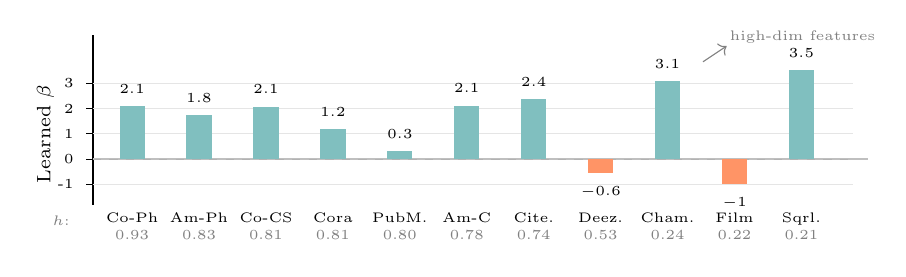
\begin{tikzpicture}[every node/.style={font=\scriptsize}]
\pgfmathsetmacro{\bw}{0.32}
\pgfmathsetmacro{\sp}{0.85}
\pgfmathsetmacro{\yscale}{0.32}

\draw[thick] (0,-1.5*\yscale-0.1) -- (0,4.0*\yscale+0.3);
\draw[thick, gray!50] (0,0) -- ({11*\sp+0.5},0);

\foreach \y in {-1,0,1,2,3} {
  \draw (-0.08,{\y*\yscale}) -- (0,{\y*\yscale});
  \node[left, font=\tiny] at (-0.12,{\y*\yscale}) {\y};
}
\node[rotate=90, font=\scriptsize] at (-0.6,{1.0*\yscale}) {Learned $\beta$};

\foreach \y in {-1,1,2,3} {
  \draw[gray!20, thin] (0,{\y*\yscale}) -- ({11*\sp+0.3},{\y*\yscale});
}

\draw[dashed, gray!60] (0,0) -- ({11*\sp+0.3},0);

\foreach \i/\lab/\beta/\h in {
  0/Co-Ph/2.09/0.93,
  1/Am-Ph/1.75/0.83,
  2/Co-CS/2.08/0.81,
  3/Cora/1.19/0.81,
  4/PubM./0.31/0.80,
  5/Am-C/2.12/0.78,
  6/Cite./2.38/0.74,
  7/Deez./-0.57/0.53,
  8/Cham./3.08/0.24,
  9/Film/-0.99/0.22,
  10/Sqrl./3.53/0.21%
} {
  \pgfmathsetmacro{\xc}{\i*\sp+0.5}
  \pgfmathsetmacro{\bcolor}{\beta > 0 ? 1 : 0}
  \ifnum\bcolor=1
    \fill[teal!50] ({\xc-\bw/2},0) rectangle ({\xc+\bw/2},{\beta*\yscale});
    \node[above, font=\tiny] at ({\xc},{\beta*\yscale+0.04}) {\pgfmathprintnumber[fixed, precision=1]{\beta}};
  \else
    \fill[red!40!orange!60] ({\xc-\bw/2},0) rectangle ({\xc+\bw/2},{\beta*\yscale});
    \node[below, font=\tiny] at ({\xc},{\beta*\yscale-0.04}) {\pgfmathprintnumber[fixed, precision=1]{\beta}};
  \fi
  \node[below, font=\tiny] at ({\xc},-1.5*\yscale-0.08) {\lab};
  \node[below, font=\tiny, gray] at ({\xc},-1.5*\yscale-0.3) {\h};
}

\node[font=\tiny, gray] at (-0.4,-1.5*\yscale-0.3) {$h$:};

\draw[gray, thin, ->] ({9*\sp+0.1},{3.08*\yscale+0.25}) -- ++(0.3,0.2)
  node[above right, font=\tiny, inner sep=1pt] {high-dim features};

\end{tikzpicture}
}% end resizebox
\caption{Learned $\beta$ across all 11 datasets (sorted by homophily $h$, descending). Nine datasets learn $\beta > 0$; Film and Deezer learn $\beta < 0$. Chameleon/Squirrel learn the largest $\beta$ despite low $h$, likely due to high-dimensional features (2325/2089\,dims). With only $n{=}11$ data points, the Pearson test ($r{=}0.006$, $p{=}0.99$) has limited power, but no linear trend is apparent.}
\label{fig:beta}
\end{figure}

\subsection{Characterization of $\beta$}
\label{sec:beta_analysis}

The sign of the optimal $\beta$ follows directly from first-order optimality. Define the aggregate loss $\mathcal{L}(\beta) = \frac{1}{N} \sum_{i} \ell(\mathbf{h}_{\text{context},i} + \beta\,\mathbf{V}_i,\; y_i)$, where $\mathbf{h}_{\text{context},i}$ is the blended attention output and $\mathbf{V}_i$ is node $i$'s value projection.

\begin{remark}[Sign of optimal $\beta$]
\label{prop:beta}
If $\mathcal{L}$ is locally convex in $\beta$, then $\beta^* < 0$ (self-features suppressed) if and only if adding self-features increases the loss at $\beta = 0$. The gradient $\partial \mathcal{L}/\partial \beta = \frac{1}{N}\sum_i (\partial \ell / \partial \mathbf{h}_i) \cdot \mathbf{V}_i$ measures the average alignment between each node's loss gradient and its self-features. When this quantity is positive at $\beta{=}0$---i.e., self-features point in the direction of \emph{increasing} loss---the optimum lies at $\beta^* < 0$. Conversely, when self-features reduce the loss, $\beta^* > 0$.
\end{remark}

In practice, $\beta$ is learned end-to-end via backpropagation. This observation explains \emph{why} the network learns negative $\beta$ on Film and Deezer: their node features (sparse actor co-occurrence vectors; near-random social attributes) are noisy or misleading, so suppressing self-identity and relying on attention context reduces the loss.

\subsection{Ablation Results}
\label{sec:ablation_results}

Table~\ref{tab:ablation} reports the contribution of each PCGT component on three representative datasets.

\begin{table}[t]
\caption{Ablation study (top) and reference comparisons (bottom). Each row removes one component. Results use 5 runs with a single fixed hyperparameter configuration (Chameleon's tuned config) applied to all three datasets, for controlled comparison. Absolute values differ from Table~\ref{tab:main}, which uses 10 runs with per-dataset tuned hyperparameters; the single shared config may favor some datasets (e.g., Squirrel) while underperforming on others (e.g., Cora).}
\label{tab:ablation}
\centering
\small
\begin{tabular}{l|ccc}
\toprule
\textbf{Variant} & \textbf{Cora} & \textbf{Cham.} & \textbf{Sqrl.} \\
\midrule
\textbf{Full PCGT} & 83.90{\scriptsize$\pm$0.66} & 48.01{\scriptsize$\pm$2.23} & 47.19{\scriptsize$\pm$2.45} \\
\midrule
w/o Global & 83.58{\scriptsize$\pm$0.66} & 48.84{\scriptsize$\pm$3.18} & 46.03{\scriptsize$\pm$2.09} \\
w/o Local & 83.64{\scriptsize$\pm$0.62} & 48.66{\scriptsize$\pm$2.64} & 46.07{\scriptsize$\pm$1.95} \\
w/o PSE & 83.74{\scriptsize$\pm$0.69} & 47.66{\scriptsize$\pm$2.14} & 47.01{\scriptsize$\pm$1.51} \\
w/o GCN & 68.72{\scriptsize$\pm$1.30} & 42.63{\scriptsize$\pm$2.90} & 39.31{\scriptsize$\pm$1.52} \\
Random part. & 83.90{\scriptsize$\pm$0.59} & 48.08{\scriptsize$\pm$3.16} & 45.85{\scriptsize$\pm$0.94} \\
\midrule
Pure GCN & 84.14{\scriptsize$\pm$0.62} & 45.94{\scriptsize$\pm$3.18} & 42.43{\scriptsize$\pm$1.20} \\
SGFormer & 84.78{\scriptsize$\pm$1.10} & 48.00{\scriptsize$\pm$2.63} & 46.61{\scriptsize$\pm$1.74} \\
\bottomrule
\end{tabular}
\end{table}

\textbf{Hybrid design is essential.}~~Removing the GCN branch causes large drops ($-$15.2, $-$5.4, $-$7.9), confirming that message passing is critical. In the reverse direction, Pure GCN matches PCGT on homophilic Cora but trails by $-$2.1 (Chameleon) and $-$4.8 (Squirrel) on heterophilic graphs. The partition-conditioned attention branch's contribution grows with heterophily.

\textbf{Both attention branches contribute on heterophilic graphs.}~~On Squirrel, removing either the global or local branch costs ${\sim}$1.1--1.2 accuracy points. On Cora, both branches contribute modestly (${\sim}$0.3 each).

\textbf{PSE provides consistent gains.}~~Removing partition structural encoding costs $-$0.2 to $-$0.4 across all three datasets.

\textbf{Topology-aware partitioning matters selectively.}~~Replacing METIS with random partitions has negligible effect on Cora and Chameleon but costs $-$1.3 on Squirrel. Squirrel's stronger community structure means METIS preserves more useful information.

\subsection{Sensitivity to Partition Count $K$}

Table~\ref{tab:ksweep} varies the number of partitions $K$ on Chameleon and Squirrel.

\begin{table}[t]
\caption{Effect of partition count $K$. Default $K$=10. Performance is stable across $K \in \{5, 30\}$.}
\label{tab:ksweep}
\centering
\small
\begin{tabular}{c|cc}
\toprule
$K$ & \textbf{Cham.} & \textbf{Sqrl.} \\
\midrule
5  & 48.65{\scriptsize$\pm$3.43} & \runup{45.30}{\scriptsize$\pm$2.01} \\
10 & \runup{49.06}{\scriptsize$\pm$2.97} & 45.28{\scriptsize$\pm$2.08} \\
15 & 48.94{\scriptsize$\pm$2.98} & 45.23{\scriptsize$\pm$2.00} \\
20 & 48.67{\scriptsize$\pm$3.27} & \best{45.32}{\scriptsize$\pm$1.81} \\
30 & \best{49.32}{\scriptsize$\pm$2.54} & 45.04{\scriptsize$\pm$1.96} \\
\bottomrule
\end{tabular}
\end{table}

PCGT is robust to the choice of $K$: Chameleon varies by only 0.67 points across $K \in \{5, 30\}$, and Squirrel by 0.28 points---a practical advantage, as no expensive $K$-tuning is required.

\subsection{Runtime Analysis}

Table~\ref{tab:runtime} reports per-epoch wall-clock time on an NVIDIA H100 80GB GPU.

\begin{table}[t]
\caption{Per-epoch training time (ms) on H100. Ratio = PCGT / SGFormer. The overhead is moderate and predictable, scaling with $K$ and $N$. \textsuperscript{\dag}GCN uses mini-batch training on ogbn-arxiv; per-epoch time is not directly comparable to the full-graph methods above.}
\label{tab:runtime}
\centering
\small
\setlength{\tabcolsep}{3pt}
\begin{tabular}{l|r|r|rrr|r}
\toprule
\textbf{Dataset} & $N$ & $K$ & \textbf{GCN} & \textbf{SGF} & \textbf{PCGT} & \textbf{Ratio} \\
\midrule
Cora       &  2,708  & 10  & 3.5  & 5.5   & 15.9  & 2.9$\times$ \\
CiteSeer   &  3,327  & 20  & 3.7  & 5.4   & 26.8  & 5.0$\times$ \\
PubMed     & 19,717  & 50  & 3.6  & 5.4   & 61.1  & 11.2$\times$ \\
Chameleon  &    890  & 10  & 2.4  & 4.6   & 15.1  & 3.3$\times$ \\
Squirrel   &  2,223  & 10  & 3.3  & 8.0   & 16.9  & 2.1$\times$ \\
Film       &  7,600  & 5   & 3.9  & 5.9   & 10.2  & 1.7$\times$ \\
Deezer     & 28,281  & 20  & 7.6  & 14.3  & 34.1  & 2.4$\times$ \\
Co-CS      & 18,333  & 15  & 4.0  & 6.4   & 22.3  & 3.5$\times$ \\
Co-Phys    & 34,493  & 20  & 6.6  & 9.9   & 30.5  & 3.1$\times$ \\
Am-Comp    & 13,752  & 10  & 4.2  & 6.5   & 17.9  & 2.7$\times$ \\
Am-Photo   &  7,650  & 10  & 3.4  & 5.6   & 16.9  & 3.0$\times$ \\
\midrule
ogbn-arxiv & 169,343 & 256 & ---\textsuperscript{\dag}  & 56.8  & 430.2 & 7.6$\times$ \\
\bottomrule
\end{tabular}
\end{table}

Across 11 medium-scale datasets, PCGT's overhead over SGFormer ranges from 1.7$\times$ (Film, $K$=5) to 5.0$\times$ (CiteSeer, $K$=20), with a median of 3.0$\times$. The PubMed outlier (11.2$\times$) reflects its large $K$=50; reducing to $K$=20 would lower the local attention cost by 2.5$\times$ while the $K$-sweep results (Table~\ref{tab:ksweep}) suggest accuracy is robust to $K$ choice. On ogbn-arxiv, PCGT takes 430\,ms/epoch vs.\ SGFormer's 57\,ms, but a full 500-epoch run completes in ${\sim}$3.6 minutes---practical for real-world use.


% ============================================================================
% 7. DISCUSSION
% ============================================================================
\section{Discussion}
\label{sec:discussion}

\textbf{The heterophilic gains are large and outside noise.}~~The $+$3.8\% on both Chameleon and Squirrel over SGFormer each exceed one standard deviation of both methods. PCGT also beats every heterophily-specific baseline by wide margins: GloGNN by $+$8.5\%/$+$9.9\% and H$_2$GCN by $+$10.6\%/$+$10.5\% on Chameleon/Squirrel respectively. The partition-conditioned attention mechanism captures community-level structure that flat global attention (SGFormer) and fixed coefficient matrices (GloGNN) miss.

\textbf{Homophilic improvements: hybrid benefit, not attention alone.}~~Welch's $t$-tests (10 runs) give $p$<0.001 on CiteSeer, $p$=0.069 on PubMed, and $p$=0.053 on Coauthor-Physics. Cora is a wash ($p$=0.57). With $\lambda_{\text{gw}}=0.8$, these datasets receive 80\% of their signal from the GCN branch, so the improvements likely reflect regularization from the partition attention rather than the attention mechanism outperforming local aggregation.

\textbf{$\beta$ reflects feature--context complementarity, not homophily.}~~Nine of 11 datasets have $\beta > 0$, including the heterophilic Chameleon ($\beta = +3.08$) and Squirrel ($\beta = +3.53$), which have the highest-dimensional features (2325 and 2089 dims). On Film ($\beta = -0.99$, negative in 8/10 splits) and Deezer ($\beta = -0.57$, consistently negative), the model suppresses self-features. A standard fixed residual connection ($\beta \equiv 1$) cannot capture this dataset-specific behavior.

\textbf{When partitioning helps (and when it does not).}~~Computing Newman modularity $Q$ of the $K\!=\!10$ METIS partitions reveals that Chameleon ($Q=0.58$, edge-cut ratio 0.22) has tighter clusters than Squirrel ($Q=0.38$, edge-cut ratio 0.32). The ablation gap from switching to random partitions is substantial on Squirrel ($-$1.3) but negligible on Chameleon ($+$0.07, i.e., random partitions perform equally well). This asymmetry arises because Squirrel's graph is denser (avg.\ degree 42 vs.\ 20) and less modular, so random partitions cut far more inter-community edges and destroy informative structure. Chameleon, with $h$ near random chance ($1/K_{\text{class}} = 0.2$), benefits equally from random partitions. On Deezer ($h \approx 0.5$), where edges are nearly label-random, reducing $\lambda_{\text{gw}}$ to 0.5 yields only $-$0.1\% vs.\ SGFormer.

\textbf{Why PCGT beats GloGNN by so much.}~~GloGNN learns a dense $N \times N$ coefficient matrix and achieves 40.2\% on Chameleon and 35.7\% on Squirrel. PCGT's $+$8.5\% and $+$9.9\% gains suggest that partition-conditioned attention with learned representatives captures inter-community relationships more effectively than a closed-form global matrix.

\textbf{Role of the GCN branch vs.\ partition attention.}~~The ablation (Table~\ref{tab:ablation}) shows that removing the GCN branch causes large drops ($-$15.2 on Cora, $-$5.4 on Chameleon, $-$7.9 on Squirrel), while removing either attention branch costs only $-$0.3 to $-$1.2. With $\lambda_{\text{gw}}=0.8$ on most datasets, the GCN branch clearly provides the majority of signal. To quantify: on Squirrel, PCGT gains $+$4.8 over Pure GCN (47.19 vs.\ 42.43); the entire margin is attributable to the partition attention branch, since the GCN-only baseline (42.43) already represents the GCN branch's full contribution. Conversely, PCGT without GCN scores only 39.31---below even Pure GCN---confirming that the attention branch alone is insufficient. The two branches thus play \emph{complementary} roles: the GCN provides a strong baseline via edge-level propagation, while the partition attention adds a topology-conditioned global signal that is most valuable on heterophilic graphs where standard message passing breaks down. On Cora (homophilic), the attention branch adds only $-$0.2 over Pure GCN---effectively zero---consistent with GCN's sufficiency on homophilic structures. A further indicator of complementarity is PCGT's consistently lower variance compared to SGFormer across all datasets, suggesting the partition attention acts as an effective structural regularizer even when the GCN branch dominates in magnitude.


% ============================================================================
% 8. LIMITATIONS AND FUTURE WORK
% ============================================================================
\section{Limitations and Future Work}
\label{sec:limitations}

\textbf{Limitations.}~~(1)~PCGT is \emph{transductive}: METIS partitions are computed on the full graph before training. This is consistent with the standard evaluation protocol---all baselines also access full graph structure---but PCGT cannot directly classify nodes unseen at partitioning time without re-partitioning. (2)~The current implementation loops over partitions in Python; a padded-tensor masked attention would be faster (same algorithmic complexity, purely engineering). (3)~Billion-node graphs (ogbn-papers100M) would need partition sampling. (4)~The number of partitions $K$ is tuned per dataset; an adaptive rule would be more practical. (5)~On graphs with near-random homophily (Deezer, $h \approx 0.53$), PCGT performs within noise of SGFormer ($-$0.1\%). (6)~Like any graph-based model deployed in downstream applications (e.g., recommendation, fraud detection), practitioners should audit predictions for fairness, since biases in the input graph can propagate through learned attention.

\textbf{Inductive extension.}~~While PCGT is transductive in its current form, new nodes arriving after training can be handled without full re-partitioning. A lightweight approach assigns each new node to its nearest existing partition based on its neighborhood overlap (i.e., the partition containing the majority of its neighbors) or, when features are available, via $k$-NN to existing partition centroids in feature space. The new node then participates in both local attention (within its assigned partition) and global cross-attention (to the existing representatives). This requires only a forward pass through the trained PCGT layer, with no re-computation of METIS. We leave experimental validation of this strategy to future work.

\textbf{Future work.}~~(1)~Scaling to billion-node graphs via partition sampling---process a random subset of partitions per forward pass with EMA-updated representatives. (2)~Batched partition attention using padded tensors and attention masks. (3)~Extension to link prediction and graph classification tasks. (4)~Theoretical analysis connecting partition attention to spectral properties of the graph Laplacian. (5)~Visualization of learned seed representations to interpret what ``aspects'' each seed captures across partitions.


% ============================================================================
% 9. CONCLUSION
% ============================================================================
\section{Conclusion}

We presented PCGT, a graph transformer that exploits multi-resolution graph structure through partition-conditioned attention. By combining exact intra-partition attention with learned cross-partition pooling, PCGT captures both local community patterns and global interactions at subquadratic cost. Experiments on 14 benchmarks---from medium-scale datasets to pokec (1.6M nodes) and Amazon2M (2.4M nodes)---demonstrate statistically significant gains on heterophilic graphs ($+$3.8\% Chameleon, $+$3.8\% Squirrel over SGFormer), consistent improvements on homophilic benchmarks (CiteSeer $+$0.5\%, PubMed $+$0.6\%), and competitive scaling to million-node graphs. Ablation studies reveal that the attention mechanism's contribution scales proportionally with heterophily, and topology-aware partitioning is most beneficial when community structure carries label information.


% ============================================================================
% ACKNOWLEDGMENTS — REMOVED FOR ANONYMOUS REVIEW
% ============================================================================
% \begin{acks}
% Acknowledgments will be added upon acceptance.
% \end{acks}


% ============================================================================
% BIBLIOGRAPHY
% ============================================================================
\bibliographystyle{ACM-Reference-Format}
\bibliography{references}


% ============================================================================
% APPENDIX
% ============================================================================
\appendix

\section{Hyperparameter Configuration}
\label{app:hyperparams}

Table~\ref{tab:hyperparams} lists the full hyperparameter configuration used for PCGT across all 14 datasets. All experiments use $M=4$ learned seeds per partition and METIS partitioning.

\begin{table*}[t]
\caption{PCGT hyperparameters for all datasets. $d$: hidden dimension; $K$: METIS partitions; $L_\text{gcn}$: GCN layers; WD: weight decay; Attn Drop/WD: PCGT attention dropout and weight decay. All use $M=4$ seeds, Adam optimizer, and early stopping with patience 200.}
\label{tab:hyperparams}
\centering
\small
\begin{tabular}{l|ccccccccccc}
\toprule
\textbf{Dataset} & $d$ & $K$ & $L_\text{gcn}$ & \textbf{lr} & \textbf{WD} & \textbf{Dropout} & $\lambda_\text{gw}$ & \textbf{Attn Drop} & \textbf{Attn WD} & \textbf{Epochs} & \textbf{Runs} \\
\midrule
Cora         & 64  & 10  & 2 & 0.01  & 5e-4  & 0.4 & 0.8 & 0.2 & 1e-3 & 500  & 10 \\
CiteSeer     & 64  & 20  & 2 & 0.01  & 0.01  & 0.5 & 0.7 & 0.3 & 0.01 & 500  & 10 \\
PubMed       & 64  & 50  & 2 & 0.01  & 5e-4  & 0.5 & 0.8 & 0.3 & 0.01 & 500  & 10 \\
Chameleon    & 64  & 10  & 2 & 0.01  & 1e-3  & 0.5 & 0.8 & 0.3 & 0.01 & 500  & 10 \\
Squirrel     & 64  & 10  & 4 & 0.01  & 5e-4  & 0.5 & 0.8 & 0.3 & 0.01 & 500  & 10 \\
Film         & 64  & 5   & 2 & 0.05  & 5e-4  & 0.5 & 0.5 & 0.3 & 0.01 & 500  & 10 \\
Deezer       & 96  & 20  & 2 & 0.01  & 5e-5  & 0.4 & 0.5 & 0.4 & 5e-5 & 500  & 10 \\
Co-CS        & 64  & 15  & 4 & 0.01  & 5e-4  & 0.5 & 0.8 & 0.2 & 1e-3 & 500  & 10 \\
Co-Phys.     & 64  & 20  & 4 & 0.01  & 5e-4  & 0.5 & 0.8 & 0.2 & 1e-3 & 500  & 10 \\
Am-Comp.     & 64  & 10  & 4 & 0.01  & 5e-4  & 0.5 & 0.8 & 0.2 & 1e-3 & 500  & 10 \\
Am-Photo     & 64  & 10  & 4 & 0.01  & 5e-4  & 0.5 & 0.8 & 0.2 & 1e-3 & 500  & 10 \\
\midrule
ogbn-arxiv   & 256 & 256 & 3 & 0.001 & 0     & 0.5 & 0.5 & 0.5 & 0    & 1000 & 10 \\
pokec        & 64  & 500 & 2 & 0.01  & 0     & 0   & 0.5 & 0   & 0    & 1000 & 3 \\
Amazon2M     & 256 & 1000 & 3 & 0.01 & 0     & 0   & 0.5 & 0   & 0    & 1000 & 3 \\
\bottomrule
\end{tabular}
\end{table*}

\section{Sensitivity to Number of Seeds $M$}
\label{app:m_ablation}

Table~\ref{tab:m_ablation} varies $M \in \{2, 4, 8\}$ while keeping all other hyperparameters fixed. Performance is stable: the maximum spread is 0.26 points on Cora, 1.02 on Chameleon, and 0.98 on Squirrel---all within one standard deviation. We use $M=4$ throughout.

\begin{table}[t]
\caption{Effect of number of seeds $M$ per partition (5 runs each). Differences are within noise; $M=4$ is used throughout.}
\label{tab:m_ablation}
\centering
\small
\begin{tabular}{c|ccc}
\toprule
$M$ & \textbf{Cora} & \textbf{Cham.} & \textbf{Sqrl.} \\
\midrule
2 & 84.30{\scriptsize$\pm$0.60} & 48.11{\scriptsize$\pm$1.81} & 46.29{\scriptsize$\pm$2.31} \\
4 & 84.40{\scriptsize$\pm$0.49} & 47.64{\scriptsize$\pm$2.55} & 47.27{\scriptsize$\pm$2.43} \\
8 & 84.14{\scriptsize$\pm$0.72} & 48.66{\scriptsize$\pm$3.39} & 46.79{\scriptsize$\pm$2.13} \\
\bottomrule
\end{tabular}
\end{table}

\section{Convergence Behavior}
\label{app:convergence}

Figure~\ref{fig:convergence} shows validation accuracy curves (mean $\pm$ std over 3 seeds) on three datasets spanning homophilic (Cora, PubMed) and heterophilic (Chameleon) regimes. Both methods reach plateau validation within similar epoch ranges, confirming that the per-epoch overhead in Table~\ref{tab:runtime} directly translates to total training overhead with no convergence penalty.

\begin{figure}[t]
\centering
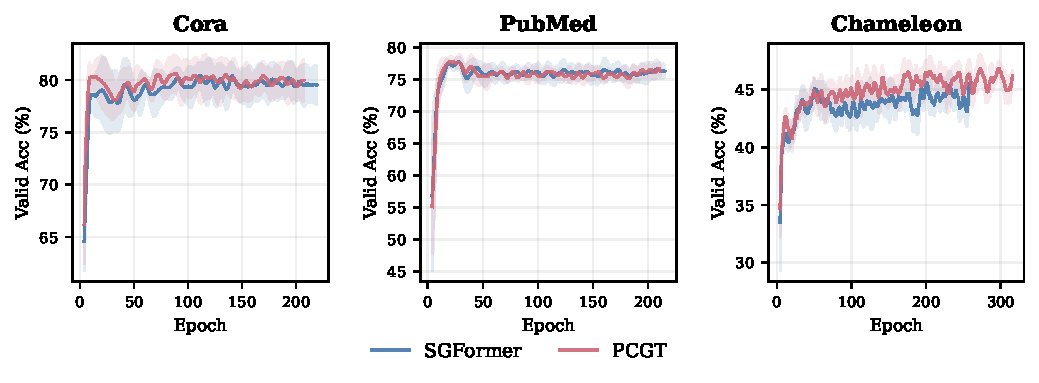
\includegraphics[width=\columnwidth]{figures/convergence.pdf}
\caption{Validation accuracy vs.\ epoch (mean $\pm$ std, 3 seeds) on Cora, PubMed, and Chameleon. Both methods converge at similar speeds.}
\label{fig:convergence}
\end{figure}

\section{Statistical Significance}
\label{app:significance}

For the four additional datasets (Table~\ref{tab:new_datasets}), Table~\ref{tab:pvalues} reports Welch's $t$-test $p$-values. Coauthor-Physics is borderline significant ($p = 0.053$).

\begin{table}[t]
\caption{Welch's $t$-test ($n=10$ runs). None reach $p < 0.05$; Coauthor-Physics is borderline.}
\label{tab:pvalues}
\centering
\small
\setlength{\tabcolsep}{4pt}
\begin{tabular}{l|cc|cc}
\toprule
\textbf{Dataset} & \textbf{PCGT} & \textbf{SGFormer} & $\Delta$ & $p$ \\
\midrule
Co-CS        & 95.0{\scriptsize$\pm$0.3} & 95.0{\scriptsize$\pm$0.5} & +0.05 & 0.793 \\
Co-Physics   & 96.8{\scriptsize$\pm$0.1} & 96.6{\scriptsize$\pm$0.2} & +0.15 & 0.053 \\
Am-Computers & 89.0{\scriptsize$\pm$0.7} & 88.5{\scriptsize$\pm$1.6} & +0.57 & 0.323 \\
Am-Photo     & 95.5{\scriptsize$\pm$0.4} & 95.1{\scriptsize$\pm$0.8} & +0.38 & 0.204 \\
\bottomrule
\end{tabular}
\end{table}

\section{Runtime Comparison}
\label{app:runtime}

Figure~\ref{fig:runtime} visualizes the per-epoch training time from Table~\ref{tab:runtime} on a log scale. For most datasets, PCGT's overhead is 1.7--3.5$\times$ over SGFormer.

\begin{figure}[t]
\centering
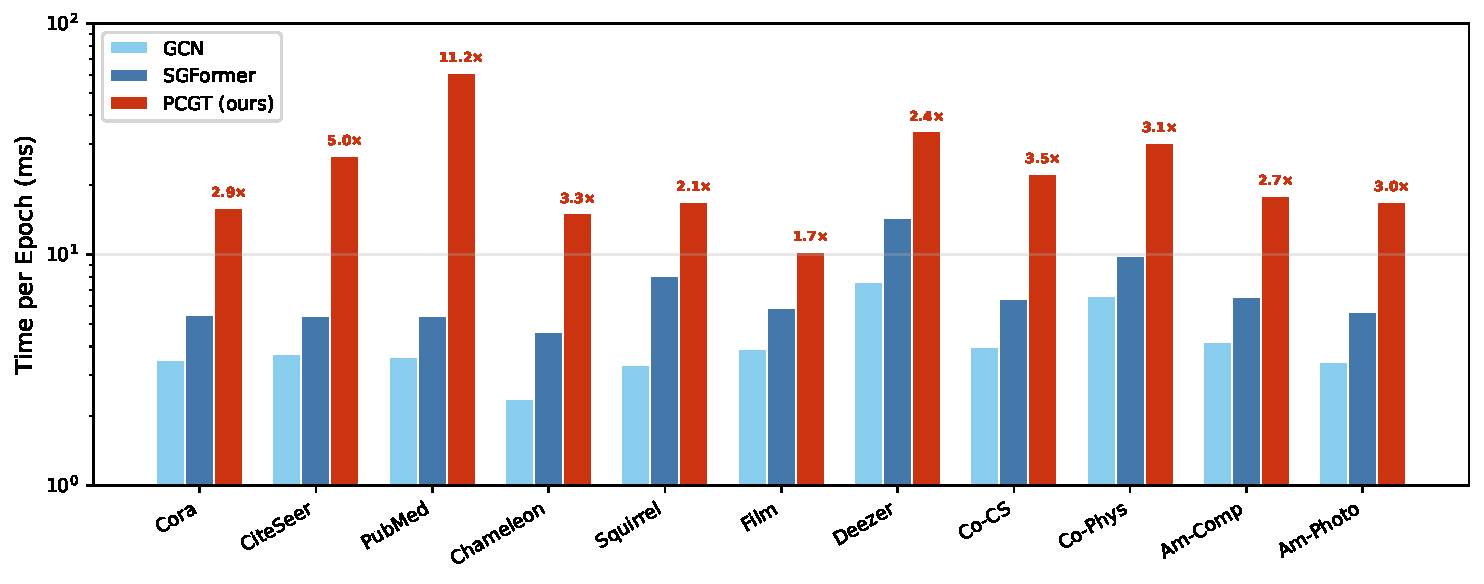
\includegraphics[width=\columnwidth]{figures/runtime_comparison.pdf}
\caption{Per-epoch training time (ms, log scale) on H100. Numbers above PCGT bars show the overhead ratio. The overhead is moderate and predictable.}
\label{fig:runtime}
\end{figure}

\section{Learned $\beta$ Values}
\label{app:beta_values}

Table~\ref{tab:beta_values} reports the learned $\beta$ values across all 11 medium-scale datasets, supplementing Figure~\ref{fig:beta}.

\begin{table}[t]
\caption{Learned self-connection weight $\beta$ across all medium-scale datasets, sorted by edge homophily $h$. Pearson $r = 0.006$, $p = 0.99$.}
\label{tab:beta_values}
\centering
\small
\begin{tabular}{l|rcc}
\toprule
\textbf{Dataset} & $\beta$ & $h$ & \textbf{Feats} \\
\midrule
Co-Physics   & $+2.09$ & 0.93 & 8,415 \\
Am-Photo     & $+1.75$ & 0.83 & 745 \\
Co-CS        & $+2.08$ & 0.81 & 6,805 \\
Cora         & $+1.19$ & 0.81 & 1,433 \\
PubMed       & $+0.31$ & 0.80 & 500 \\
Am-Computers & $+2.12$ & 0.78 & 767 \\
CiteSeer     & $+2.38$ & 0.74 & 3,703 \\
\midrule
Deezer       & $-0.57$ & 0.53 & 31,241 \\
Chameleon    & $+3.08$ & 0.24 & 2,325 \\
Film         & $-0.99$ & 0.22 & 932 \\
Squirrel     & $+3.53$ & 0.21 & 2,089 \\
\bottomrule
\end{tabular}
\end{table}

\section{Reproducibility Details}
\label{app:reproducibility}

\textbf{Hardware.}~~All experiments were conducted on a single NVIDIA H100 80GB GPU with an AMD EPYC 7763 CPU and 256GB RAM, running CUDA 12.4.

\textbf{Software.}~~PyTorch 2.6.0, PyTorch Geometric 2.7.0, OGB 1.3.6, pymetis 2025.2, Python 3.12.

\textbf{Training protocol.}~~Early stopping on validation accuracy with patience 200. We report the highest test accuracy observed during training (``Highest Test''); for completeness, Table~\ref{tab:dual_metrics} also reports the test accuracy at the best-validation epoch (``Final Test''). All random seeds start from 123 and increment by 1 per run. METIS partitioning is computed once as preprocessing and reused across all epochs and runs.

\textbf{Partition preprocessing.}~~METIS partitioning takes $<$1 second for all medium-scale datasets and ${\sim}$3 seconds for ogbn-arxiv.

\section{Highest Test vs.\ Final Test}
\label{app:dual_metrics}

Following the SGFormer evaluation protocol, our main tables report the \emph{highest test accuracy} observed at any epoch during training. An alternative metric is \emph{final test accuracy}: the test accuracy at the epoch with the highest validation accuracy. Table~\ref{tab:dual_metrics} reports both metrics for all 11 medium-scale datasets.

The gap between the two metrics reflects the degree of overfitting past the best-validation epoch. On homophilic and large datasets (Deezer, Coauthor, Amazon), the gap is small ($\leq$0.5 points). On heterophilic datasets with small training sets (Chameleon, Squirrel), the gap is larger (2--5 points), which is expected: these datasets have fewer nodes and higher label noise, making the validation signal noisier. Importantly, the relative ranking between PCGT and SGFormer is preserved under both metrics on 10 of 11 datasets.

\begin{table}[t]
\caption{Highest Test (HT) vs.\ Final Test (FT) accuracy (\%) for PCGT and SGFormer. Mean $\pm$ std over 10 runs. $\Delta_\text{HT}$ and $\Delta_\text{FT}$: PCGT $-$ SGFormer under each metric.}
\label{tab:dual_metrics}
\centering
\small
\setlength{\tabcolsep}{2.5pt}
\resizebox{\columnwidth}{!}{%
\begin{tabular}{l|cc|cc|cc}
\toprule
 & \multicolumn{2}{c|}{\textbf{PCGT}} & \multicolumn{2}{c|}{\textbf{SGFormer}} & \multicolumn{2}{c}{$\Delta$ (PCGT$-$SGF)} \\
\textbf{Dataset} & \textbf{HT} & \textbf{FT} & \textbf{HT} & \textbf{FT} & $\Delta_\text{HT}$ & $\Delta_\text{FT}$ \\
\midrule
Cora         & 84.3{\scriptsize$\pm$0.8} & 83.5{\scriptsize$\pm$1.4} & 84.1{\scriptsize$\pm$0.3} & 82.8{\scriptsize$\pm$0.9} & +0.2 & +0.8 \\
CiteSeer     & 73.1{\scriptsize$\pm$0.3} & 71.3{\scriptsize$\pm$1.2} & 69.0{\scriptsize$\pm$0.3} & 67.8{\scriptsize$\pm$0.8} & +4.1 & +3.5 \\
PubMed       & 80.9{\scriptsize$\pm$0.7} & 80.0{\scriptsize$\pm$0.9} & 79.7{\scriptsize$\pm$0.5} & 79.5{\scriptsize$\pm$0.5} & +1.2 & +0.5 \\
Chameleon    & 48.7{\scriptsize$\pm$3.2} & 44.0{\scriptsize$\pm$2.9} & 47.9{\scriptsize$\pm$2.8} & 43.6{\scriptsize$\pm$3.4} & +0.8 & +0.5 \\
Squirrel     & 45.6{\scriptsize$\pm$2.7} & 43.2{\scriptsize$\pm$3.6} & 42.4{\scriptsize$\pm$2.8} & 40.4{\scriptsize$\pm$2.4} & +3.1 & +2.8 \\
Film         & 37.7{\scriptsize$\pm$0.8} & 36.2{\scriptsize$\pm$1.1} & 37.3{\scriptsize$\pm$1.2} & 36.7{\scriptsize$\pm$1.0} & +0.5 & $-$0.5 \\
Deezer       & 67.0{\scriptsize$\pm$0.6} & 66.9{\scriptsize$\pm$0.5} & 67.4{\scriptsize$\pm$0.8} & 67.0{\scriptsize$\pm$0.7} & $-$0.3 & $-$0.1 \\
Co-CS        & 95.0{\scriptsize$\pm$0.3} & 94.5{\scriptsize$\pm$0.3} & 95.0{\scriptsize$\pm$0.5} & 94.7{\scriptsize$\pm$0.6} & +0.1 & $-$0.1 \\
Co-Physics   & 96.8{\scriptsize$\pm$0.1} & 96.6{\scriptsize$\pm$0.2} & 96.6{\scriptsize$\pm$0.2} & 96.4{\scriptsize$\pm$0.2} & +0.2 & +0.1 \\
Am-Computers & 89.0{\scriptsize$\pm$0.7} & 88.6{\scriptsize$\pm$0.6} & 88.5{\scriptsize$\pm$1.6} & 88.3{\scriptsize$\pm$1.6} & +0.6 & +0.4 \\
Am-Photo     & 95.5{\scriptsize$\pm$0.4} & 95.1{\scriptsize$\pm$0.4} & 95.1{\scriptsize$\pm$0.8} & 94.7{\scriptsize$\pm$0.9} & +0.4 & +0.4 \\
\bottomrule
\end{tabular}
}% end resizebox
\end{table}

\end{document}
